\documentclass[letterpaper,12pt]{article}
\usepackage[spanish]{babel}
\spanishdecimal{.}
\usepackage[utf8]{inputenc}
\usepackage{graphicx}
\usepackage[top=2.5cm, bottom=2.5cm, left=2.5cm, right=2.5cm]{geometry}
\usepackage{hyperref}
\usepackage{verbatim}

\title{Práctica 2 \\ Instalación de software para operar robots móviles}
\author{M.I. Marco Negrete}
\date{Robots Móviles y Agentes Inteligentes}
\begin{document}
\renewcommand{\tablename}{Tabla}
\maketitle
\section*{Objetivos}
\begin{itemize}
\item Familiarizar al alumno con el uso del software de control de versiones \texttt{git}.
\item Aprender a utilizar el software desarrollado en el Laboratorio de Biorrobótica para la operación de robots móviles autónomos. 
\end{itemize}

\section{Introducción}
\textbf{Git.} Es un software de control de versiones \textit{open source}, creado por Linus Torvalds. Está pensado para el desarrollo de software cuando éste posee una gran cantidad de código fuente y facilita el trabajo cooperativo mediante el manejo de \textit{branching} y herramientas de solución de conflictos. 

En este curso se usará \texttt{git} para el manejo de versiones del software necesario para operar los robots que se utilizarán en el desarrollo de prácticas y proyectos. Además, proporcionará al alumno herramientas para desarrollar de forma ordenada todos los códigos necesarios.

En la página \url{https://git-scm.com/} se pueden encontrar tutoriales para aprender más sobre \texttt{git}.

\textbf{Justina.} Es un robot de servicio desarrollado en el Laboratorio de Biorrobótica de la Facultad de Ingeniería de la UNAM. En este curso se utilizarán algunos de los paquetes de ROS del software de Justina. 

\section{Desarrollo}
\subsection{Instalación de Git y obtención del software}
\textbf{Nota.} Se asume que el alumno ya tiene instalado Ubuntu 14.04 y ROS Indigo. 

En una terminal, teclear los siguientes comandos:
\begin{verbatim}
sudo apt-get install git
cd ~
git clone https://github.com/mnegretev/RoboticsCourses.git
\end{verbatim}
Lo anterior descarga una copia del repositorio que contiene el material a usar durante el curso. Para descargar una actualización, teclee el siguiente comando:
\begin{verbatim}
git pull origin master
\end{verbatim}
Puesto que en este momento no hay ninguna actualización disponible, se debe leer la siguiente salida:
\begin{verbatim}
From https://github.com/mnegretev/RoboticsCourses
 * branch            master    -> FETCH_HEAD
Already up-to-date.
\end{verbatim}

\subsection{Instalación de dependencias y compilación}
Para poder compilar y ejecutar el software, es necesario instalar varias dependencias. Para ello, en una terminal teclee los siguientes comandos:
\begin{verbatim}
cd ~/RoboticsCourses
./Setup.sh
\end{verbatim}

Esto comenzará a instalar varias bibliotecas como OpenCV (software para visión computacional), PCL (procesamiento de nubes de puntos), PrimeSense (controladores para cámaras RGB-D) y algunos paquetes de ROS necesarios. Cuando el script termine de ejecutarse, teclee los siguientes comandos para compilar el código:
\begin{verbatim}
cd ~/RoboticsCourses/catkin_ws
catkin_make
\end{verbatim}

Una vez finalizada la compilación, ejecute los siguientes comandos:

\begin{verbatim}
cd ~/RoboticsCourses/catkin_ws
source devel/setup.bash
roslaunch bring_up hardware_simul.launch
\end{verbatim}

Se mostrará una ventana como la que se observa en la figura \ref{fig:rviz}.
\begin{figure}
\centering
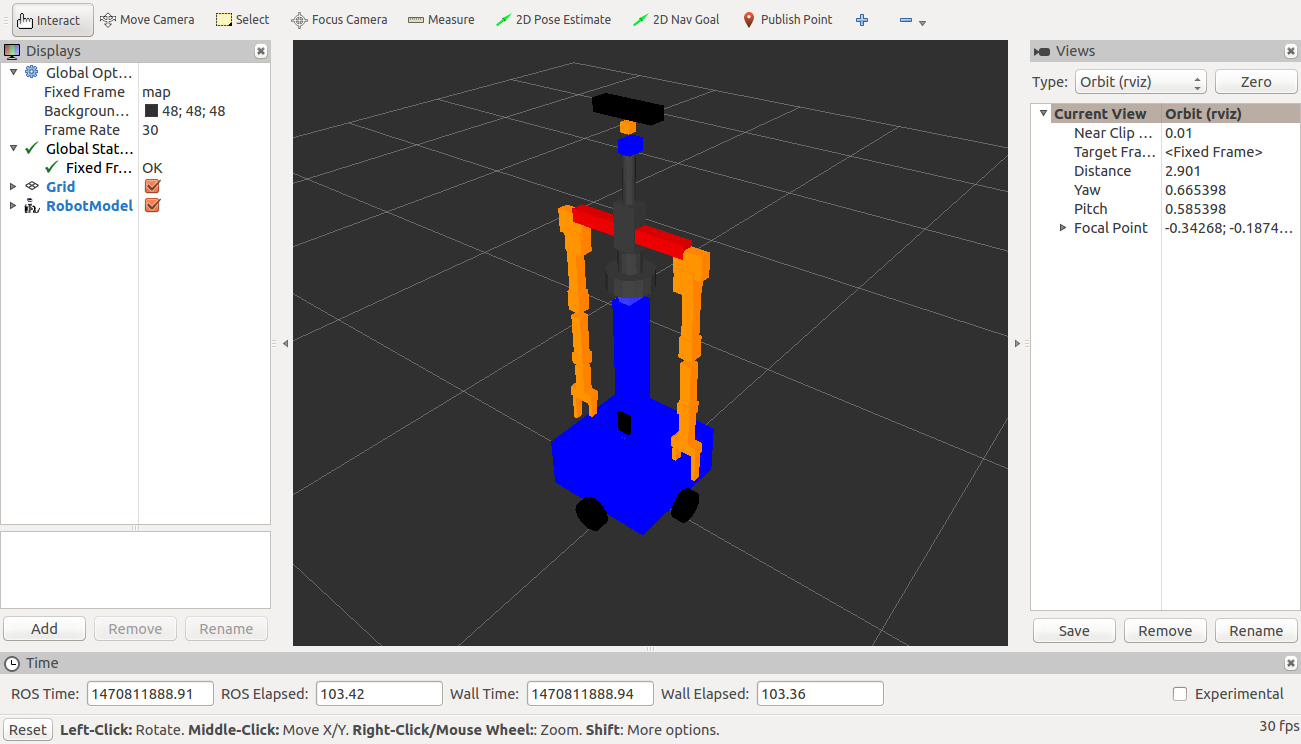
\includegraphics[width=0.8\textwidth]{rviz_initial.png}
\caption{El visualizador \texttt{rviz}}
\label{fig:rviz}
\end{figure}
\end{document}